\documentclass{article}
\usepackage{graphicx}
\usepackage{subcaption}
\usepackage{wrapfig}
\title{Insert Add in Latex}
\author{MD Hasib Mia}
\begin{document}
	\maketitle
	\tableofcontents
	\clearpage
	
	\section{Add Single Image:}
	\begin{figure}[htp]              %-----------------this use for insert image at inserted position
		\centering  %---------------left shift: \raggedright . Right shift: \raggedleft
		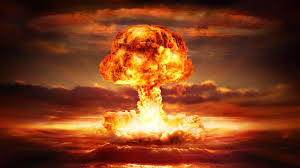
\includegraphics[width=.5\textwidth]{first.jpg}
		\caption{Atom Bomb}
	\end{figure}
	
	
	
	\section{Insert two image:}
    \begin{figure}[htbp]
	\centering
		% First subfigure
	\begin{subfigure}[b]{0.4\textwidth} % -------------> Set the width of the first subfigure
		\centering
		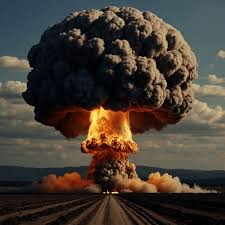
\includegraphics[height=.73\textwidth]{second.jpg}
		\caption{2nd photo}
		\label{fig:second}
	\end{subfigure}
	\hspace{0.05\textwidth} % ------------space between two image
	\begin{subfigure}[b]{0.4\textwidth} % ------------>Set the width of the subfigure
		\centering
		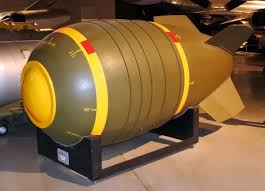
\includegraphics[width=\textwidth]{third.jpg}
		\caption{3rd photo}
		\label{fig:third}
	\end{subfigure}
	\caption{Example of two subfigures}
	\label{fig:example}
\end{figure}

\clearpage




%--------------------------------------------wrapping text with image---------------------------------
\section{Wrapping text with image }
An atom bomb, or nuclear bomb, is a powerful weapon that derives its destructive force from nuclear reactions. These reactions release immense amounts of energy by splitting (fission) or combining (fusion) atomic nuclei. The first atom bombs were developed during World War II as part of the Manhattan Project, a top-secret research initiative led by the United States.
\begin{wrapfigure}{l}{0.4\textwidth} % 'r' for right, 'l' for left
	\centering
	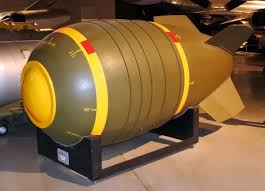
\includegraphics[width=0.38\textwidth]{third.jpg}
	\caption{Atom Bomb}
	\label{fig:wrapfig}
\end{wrapfigure}





The two most notable instances of atom bomb use occurred in August 1945, when the U.S. dropped bombs on the Japanese cities of Hiroshima and Nagasaki. The bomb dropped on Hiroshima, named Little Boy, used uranium-235 and caused massive destruction and loss of life. Three days later, the bomb dropped on Nagasaki, called Fat Man, used plutonium-239 and had similarly devastating effects. Together, these bombings resulted in the deaths of over 200,000 people, many of whom were civilians.

The development and use of atom bombs ushered in the nuclear age, fundamentally changing warfare, international relations, and global security. While they have not been used in conflict since World War II, thousands of nuclear weapons exist today, posing an ongoing threat to humanity.

Modern discussions about nuclear weapons often focus on disarmament and the prevention of proliferation. The Treaty on the Non-Proliferation of Nuclear Weapons (NPT) is an international effort to prevent the spread of nuclear weapons and promote peaceful uses of nuclear energy.


	
	
	
	
	
\end{document}